% Using Free and Open Source Solutions in Geospatial Science Education
% This work by Vaclav Petras is licensed under
% a Creative Commons Attribution-ShareAlike 4.0 International License.

% Session
%
% NS52A: A Tour of Open-Source Software Packages for the Geosciences II
%
% This session will be a rapid-fire tour of open source tools freely available for
% researchers in the geosciences. The fast-growing open-source software ecosystem
% is creating new tools and changing paradigms for how computers and
% collaborations are used to study Earth processes. If you have written
% open-source software that could be useful to others, we look forward to seeing
% your submission. This session will not only be an opportunity to showcase your
% own packages and learn about other available tools, we also hope it will be an
% opportunity to connect with others working on related problems and lead to new
% collaborations. The session will be accompanied by posters where the audience
% can engage individually with the presenters.
%
% Abstract
%
% GRASS GIS (grass.osgeo.org) is an open source software for geospatial analysis,
% remote sensing, general geoprocessing and visualization. It is a
% community-driven project with over 35 years of continuous software development
% based on scientific expertise from many geospatial fields. It is characterized
% by long-term releases, stable APIs, and emphasis on science. GRASS GIS
% distribution strives to provide single integrated environment for 2D and 3D
% raster analysis, image processing, vector data analysis, and spatio-temporal
% data processing. It supports large raster files (billions of cells), vector
% topology, coupling with databases, and 64 bit memory. New code based on recent
% research is typically contributed to GRASS GIS Addons repository. Mature, widely
% used code is then moved to the main code base to maximize integration and
% availability. Whether it is addons or the main code base, code is usually
% maintained by the community and preserved in long term even in cases when the
% original author no longer supports the code. To support the needs of scientists,
% the documentation includes not only links to the source code, its history, and
% its authors, but also links to research papers that describe the algorithms
% implemented in the modules.
%
% Code is not only maintained but also extended and improved. For example,
% watershed and stream extraction using least cost path approach was implemented
% in 1989 and extended for massive datasets in 2011. Similarly, vector topology
% cleaning was introduced in 2002, updated over time and substantially improved in
% 2016. Another example is a solar energy module available since 1993 and
% parallelized in 2017. The current stable version of GRASS GIS 7.4 provides new
% features for geosciences such as temporal framework with temporal algebra for
% large time-series processing, fusion of elevation models from various sensors,
% 3D flows, landform detection, image segmentation, simplified batch processing,
% and integrated Python editor among others. GRASS GIS runs in various
% environments including Linux, Mac, Windows, Docker, Raspberry Pi, and on HPC
% clusters. The modules are written in Python, C, or C++. Besides command line
% interface, GRASS GIS provides a graphical user interface, a Python API, and a C
% API. Interfaces with other languages such as R and Ruby are supplied by
% collaborating communities.

\documentclass[xcolor={dvipsnames,usenames},beamer,aspectratio=169]{beamer}
% ,handout,notes=show

\makeatletter
\def\beamer@framenotesbegin{% at beginning of slide
  \gdef\beamer@noteitems{}%
  \gdef\beamer@notes{{}}% used to be totally empty.
}
\makeatother

\usepackage{textcomp}
\usepackage[utf8]{inputenc}
\usepackage[american]{babel}
\usepackage{graphicx}
\usepackage{url}
\usepackage{amssymb}

\usepackage{alltt}

\usepackage{tikz}
\usetikzlibrary{arrows,shapes,spy,calc}

\tikzstyle{every picture}+=[remember picture]
\tikzstyle{na} = [baseline=-.5ex]

% don't count bacup slides
\newcommand{\backupbegin}{
   \newcounter{finalframe}
   \setcounter{finalframe}{\value{framenumber}}
}
\newcommand{\backupend}{
   \setcounter{framenumber}{\value{finalframe}}
}

% frames have to be fragile
\newif\ifnotes
% % \notestrue

% \notestrue


\ifnotes
\setbeamertemplate{note page}[plain]
% \setbeamertemplate{note page}[compress]
\setbeamerfont{note page}{size=\large}
% \setbeameroption{show only notes}
\setbeameroption{show notes}
\usepackage{pgfpages}
\pgfpagesuselayout{2 on 1}[a4paper,border shrink=5mm]%
\else
%\setbeameroption{hide notes}
\fi
%\notesfalse

\usepackage[absolute,overlay]{textpos}

\usepackage{listings}

% Fira Sans, GRASS GIS branding sans serif font
\usepackage{FiraSans}
\renewcommand*\oldstylenums[1]{{\firaoldstyle #1}}

% \usetheme{Warsaw}
\usetheme{Madrid}
% \usetheme{Frankfurt}
% \useoutertheme{infolines}
\definecolor{GRASSGISGreen}{HTML}{009000}
\usecolortheme[named=GRASSGISGreen]{structure}
\setbeamertemplate{navigation symbols}{}

\setbeamertemplate{itemize items}[default]
\setbeamertemplate{enumerate items}[default]
% \useinnertheme{rectangles}
\setbeamertemplate{blocks}[default]


%%%%%%%%%%%%%%%%%%%%%%%%%%%%%%%%%%%%%%%%%%%%%%%%%%%%%%%%%%%%%%%%%%%%
%%%%%%%%%%%%%%%%%%%%%%%%%%%%%%%%%%%%%%%%%%%%%%%%%%%%%%%%%%%%%%%%%%%%

% \newcommand{\n}[1]{$^{\color{gray}{\mbox{\tiny#1}}}$}
\newcommand{\n}[1]{$^{\textcolor{gray}{\mbox{\tiny #1}}}$}

%%%%%%%%%%%%%%%%%%%%%%%%%%%%%%%%%%%%%%%%%%%%%%%%%%%%%%%%%%%%%%%%%%%%%%%%%%%%%%%
\newcommand{\gmodule}[1]{\href{http://grass.osgeo.org/grass74/manuals/#1.html}{\emph{#1}}}
\newcommand{\amodule}[1]{\href{http://grass.osgeo.org/grass74/manuals/addons/#1.html}{\emph{#1}}}
\newcommand{\module}[1]{\emph{#1}}
\newcommand{\grasslink}{\href{http://grass.osgeo.org/}{GRASS GIS}}

%%%%%%%%%%%%%%%%%%%%%%%%%%%%%%%%%%%%%%%%%%%%%%%%%%%%%%%%%%%%%%%%%%%%
%%%%%%%%%%%%%%%%%%%%%%%%%%%%%%%%%%%%%%%%%%%%%%%%%%%%%%%%%%%%%%%%%%%%

\title[GRASS GIS]{\textbf{GRASS}\,{\firalight GIS}: A General-purpose Geospatial Research Tool}
\subtitle{
AGU 2018 Fall Meeting
\\
\scriptsize
NS52A: A Tour of Open-Source Software Packages for the Geosciences II
}
%\pdforstring{}{}

\newcommand{\inst}[1]{\hspace{2pt}$^{\mbox{\normalsize#1}}$\hspace{-7pt}}
\newcommand{\instlist}[1]{\hspace{1pt}$^{\mbox{#1}}$\hspace{0pt}}

\author[Vaclav Petras]{
Helena Mitasova\inst{1},
Vaclav Petras\inst{1}\,*\hspace{-0.2ex},
Anna Petrasova\inst{1}
\&
Markus Neteler\hspace{0.05em}\inst{2}
\\
Scientific Team: GRASS GIS Development Team**
}

\institute[NC State University]
{%
\instlist{1}Center for Geospatial Analytics, NCSU, USA;
\instlist{2}mundialis, Germany
\\
*\texttt{wenzeslaus@gmail.com, vpetras@ncsu.edu, @vaclavpetras}
\\
% using Black Duck Open Hub to ``guestimate'' that
**Includes over 10 other members of the core team and numerous other contributors

\bigskip

\includegraphics[height=0.04\textwidth]{ncstate}%
~

\includegraphics[height=0.06\textwidth]{mundialis}%
}

\date{December 14, 2018}

\setbeamercovered{transparent}

\hypersetup{%
 pdfauthor={Vaclav Petras},%
 pdfsubject={Point clouds and GRASS GIS talk at ISPRS 2016},%
 pdfkeywords={3D rasters} {decimation} {sampling} {binning}
   {LAS} {PDAL} {PCL} {Kinect}
   {v.in.lidar} {r.in.lidar} {r.in.kinect} {libLAS}
   {geospatial modeling}
   {free software} {open source} {open science}
}

\usepackage{tipa}
\newcommand{\pron}[2]{#1 [#2]}


%%%%%%%%%%%%%%%%%%%%%%%%%%%%%%%%%%%%%%%%%%%%%%%%%%%%%%%%%%%%%%%%%%%%
% when images are placed in these directories, we don't have to specify the directory
% just the filename
\graphicspath{{logos/}{images/}}


%%%%%%%%%%%%%%%%%%%%%%%%%%%%%%%%%%%%%%%%%%%%%%%%%%%%%%%%%%%%%%%%%%%%
%%%%%%%%%%%%%%%%%%%%%%%%%%%%%%%%%%%%%%%%%%%%%%%%%%%%%%%%%%%%%%%%%%%%
%%%%%%%%%%%%%%%%%%%%%%%%%%%%%%%%%%%%%%%%%%%%%%%%%%%%%%%%%%%%%%%%%%%%
%%%%%%%%%%%%%%%%%%%%%%%%%%%%%%%%%%%%%%%%%%%%%%%%%%%%%%%%%%%%%%%%%%%%
\begin{document}

\newcommand{\logowidth}{1.0em}
\newcommand{\logospace}{\hspace{0.2em}}
\newcommand{\includecclogo}[1]{\includegraphics[width=\logowidth]{#1}}

%%%%%%%%%%%%%%%%%%%%%%%%%%%%%%%%%%%%%%%%%%%%%%%%%%%%%%%%%%%%%%%%%%%%
\frame{
\titlepage
\begin{center}
\vspace{-3ex}
\href{http://creativecommons.org/licenses/by-sa/4.0/}{
\includecclogo{cc}
\logospace
\includecclogo{by}
\logospace
\includecclogo{sa}
}
\end{center}
}


%%%%%%%%%%%%%%%%%%%%%%%%%%%%%%%%%%%%%%%%%%%%%%%%%%%%%%%%%%%%%%%%%%%%%
\begin{frame}{GRASS GIS}

\begin{columns}
\begin{column}{0.74\textwidth}

\begin{itemize}
  \item all in one
  \begin{itemize}
   \item hydrology, remote sensing, network analysis, \ldots
  \end{itemize}
  \item driven by needs of users
  \begin{itemize}
   \item community has a direct access to the development process
  \end{itemize}
  \item from small laptops to supercomputers
  \begin{itemize}
   \item Raspberry Pi, Windows, macOS, GNU/Linux, FreeBSD, AIX, \ldots
  \end{itemize}
  \item learn now, use forever
  \begin{itemize}
    \item 35 years of development, many old scripts still running, \ldots
  \end{itemize}
\end{itemize}
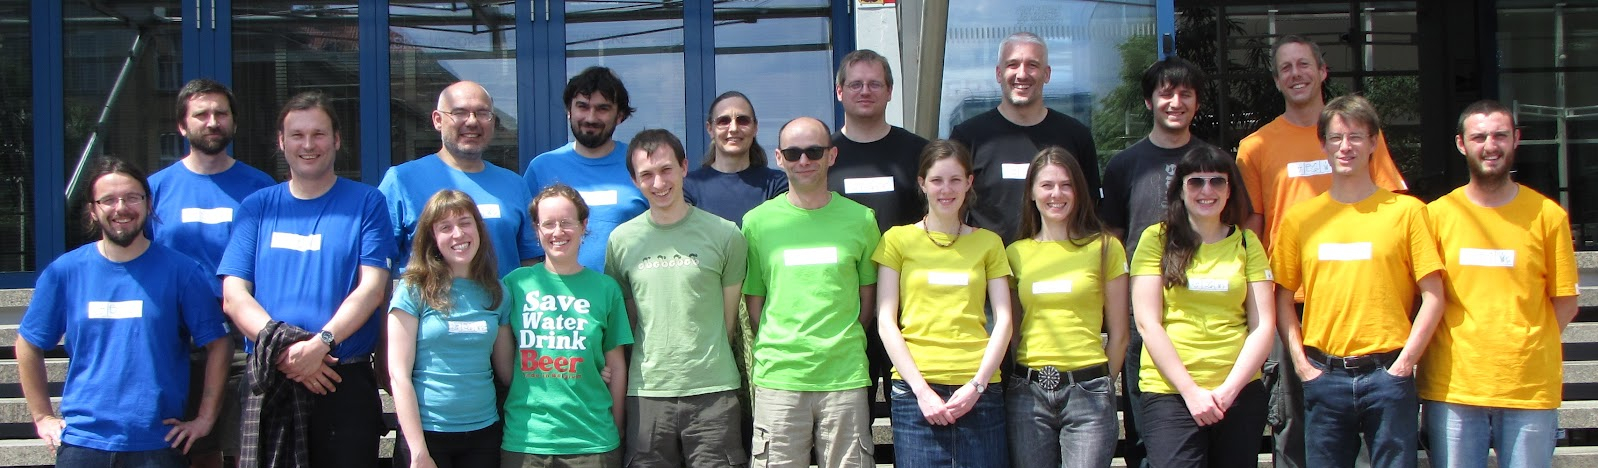
\includegraphics[width=\textwidth]{grass_team}
\end{column}
\begin{column}{0.25\textwidth}

\begin{center}
  
\includegraphics[width=\textwidth]{logos/grass_gis}
\end{center}

\vspace*{-2.5ex}

\textcolor{gray}{
\scriptsize
latest release 7.4.3
\tiny
(Nov 26, 2018)
}

\end{column}
\end{columns}

\end{frame}

%%%%%%%%%%%%%%%%%%%%%%%%%%%%%%%%%%%%%%%%%%%%%%%%%%%%%%%%%%%%%%%%%%%%%
\begin{frame}{Novel methods are published through GRASS GIS}

\begin{columns}
\begin{column}{0.5\textwidth}

\begin{itemize}
  \item temporal framework (Gebbert \& Pebesma 2014)
  \item spatio-temporal algebra (Gebbert \& Leppelt 2015)
  \item landform detection with geomorphons (Jasiewicz \& Stepinski 2013)
\end{itemize}

\bigskip
\footnoterule
\tiny

Gebbert, S. and Leppelt, T. (2015). GRASS GIS: The first Open Source Temporal GIS. In EGU General Assembly Conference Abstracts, volume 17, page 7296.

Gebbert, S. and Pebesma, E. (2014). A temporal GIS for field based environmental modeling. Environmental Modelling \& Software, 53:1–12.

Jasiewicz, J. and Stepinski, T. (2013). Geomorphons - a pattern recognition approach to classification and mapping of landforms, Geomorphology, vol. 182, 147-156. DOI~10.1016/j.geomorph.2012.11.005

\end{column}
\begin{column}{0.5\textwidth}
\centering
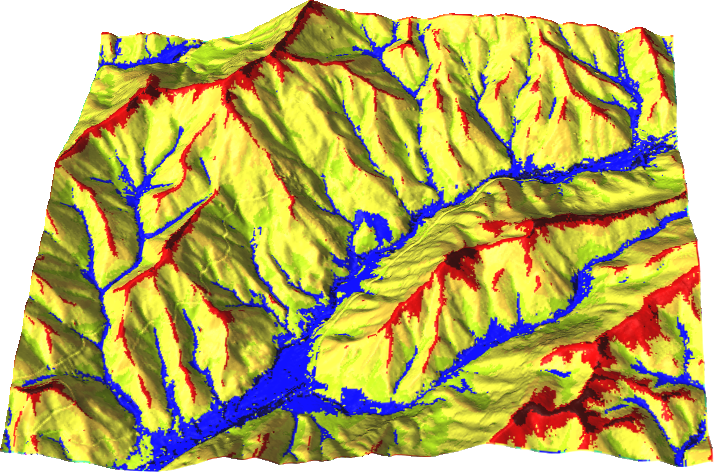
\includegraphics[width=\textwidth]{geomorphon_3d}

\textcolor{gray}{
\footnotesize
Landforms detected by \gmodule{r.geomorphon}
}

\end{column}
\end{columns}

\end{frame}


%%%%%%%%%%%%%%%%%%%%%%%%%%%%%%%%%%%%%%%%%%%%%%%%%%%%%%%%%%%%%%%%%%%%%
\begin{frame}{Research software is preserved over time}

\begin{columns}
\begin{column}{0.5\textwidth}

\begin{itemize}
  \item water flow simulation (Mitasova et al. 2004)
  \item least cost path watershed and flow tracing (Ehlschlaeger 1989)
  \item wildfire spread model (Xu 1994)
% It has
% been extensively tested and recently adapted to European fuel types (Rodriguez-Aseretto et al., 2013 [23]; de
% Rigo et al., 2013 [5]; Di Leo et al., 2013 [6]).
\end{itemize}

\bigskip
\footnoterule
\tiny

Mitasova, H., Thaxton, C., Hofierka, J., McLaughlin, R., Moore, A., Mitas L. (2004). Path sampling method for modeling overland water flow, sediment transport and short term terrain evolution in Open Source GIS. In: C.T. Miller, M.W. Farthing, V.G. Gray, G.F. Pinder eds., Proceedings of the XVth International Conference on Computational Methods in Water Resources (CMWR XV), June 13-17 2004, Chapel Hill, NC, USA, Elsevier, pp. 1479-1490.

Ehlschlaeger C. (1989). Using the $A^T$ Search Algorithm to Develop Hydrologic Models from Digital Elevation Data, Proceedings of International Geographic Information Systems (IGIS) Symposium '89, pp 275-281 (Baltimore, MD, 18-19 March 1989).

Xu, J. (1994). Simulating the spread of wildfires using a geographic information system and remote sensing. PhD thesis, Rutgers University, New Brunswick, New Jersey.

\end{column}
\begin{column}{0.5\textwidth}
\centering
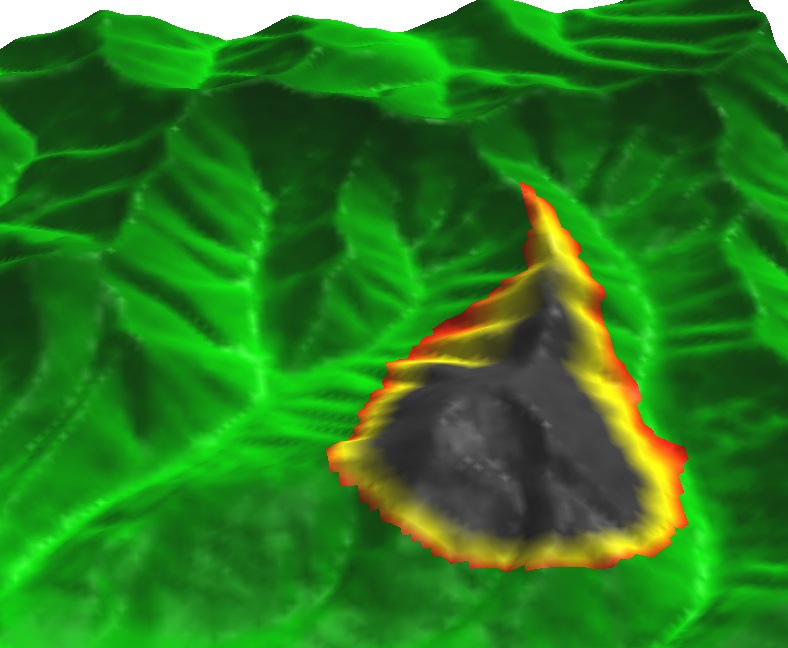
\includegraphics[width=\textwidth]{fire_spread}

\textcolor{gray}{
\footnotesize
Wildfire spread simulated by \gmodule{r.ros} and \gmodule{r.spread}
}

\end{column}
\end{columns}

\end{frame}


%%%%%%%%%%%%%%%%%%%%%%%%%%%%%%%%%%%%%%%%%%%%%%%%%%%%%%%%%%%%%%%%%%%%%
\begin{frame}{Published tools are used by other scientists}

\begin{columns}
\begin{column}{0.5\textwidth}

\begin{itemize}
  \item water flow simulation (Mitasova et al. 2004) used for emergency routing (Raghavan et al. 2014)
  \item wildfire spread model (Xu 1994) used
        for fires in Europe (Rodriguez-Aseretto et al. 2013)
%         and for travel of Vikings
\end{itemize}

\bigskip
\footnoterule
\tiny

Mitasova, H., Thaxton, C., Hofierka, J., McLaughlin, R., Moore, A., Mitas L. (2004). Path sampling method for modeling overland water flow, sediment transport and short term terrain evolution in Open Source GIS. In: C.T. Miller, M.W. Farthing, V.G. Gray, G.F. Pinder eds., Proceedings of the XVth International Conference on Computational Methods in Water Resources (CMWR XV), June 13-17 2004, Chapel Hill, NC, USA, Elsevier, pp. 1479-1490.

Raghavan, V., Choosumrong, S., Yoshida, D., and Vinayaraj, P. (2014). Deploying Dynamic Routing Service for Emergency Scenarios using pgRouting, GRASS and ZOO. In In Proceedings of FOSS4G Europe, Jacobs University, Bremen, Germany.

D. Rodriguez-Aseretto, D. de Rigo, M. Di Leo, A. Cortés, and J. San-Miguel-Ayanz (2013). A data-driven model for large wildfire behaviour prediction in Europe. Procedia Computer Science, 18:1861–1870.

\end{column}
\begin{column}{0.5\textwidth}
\centering
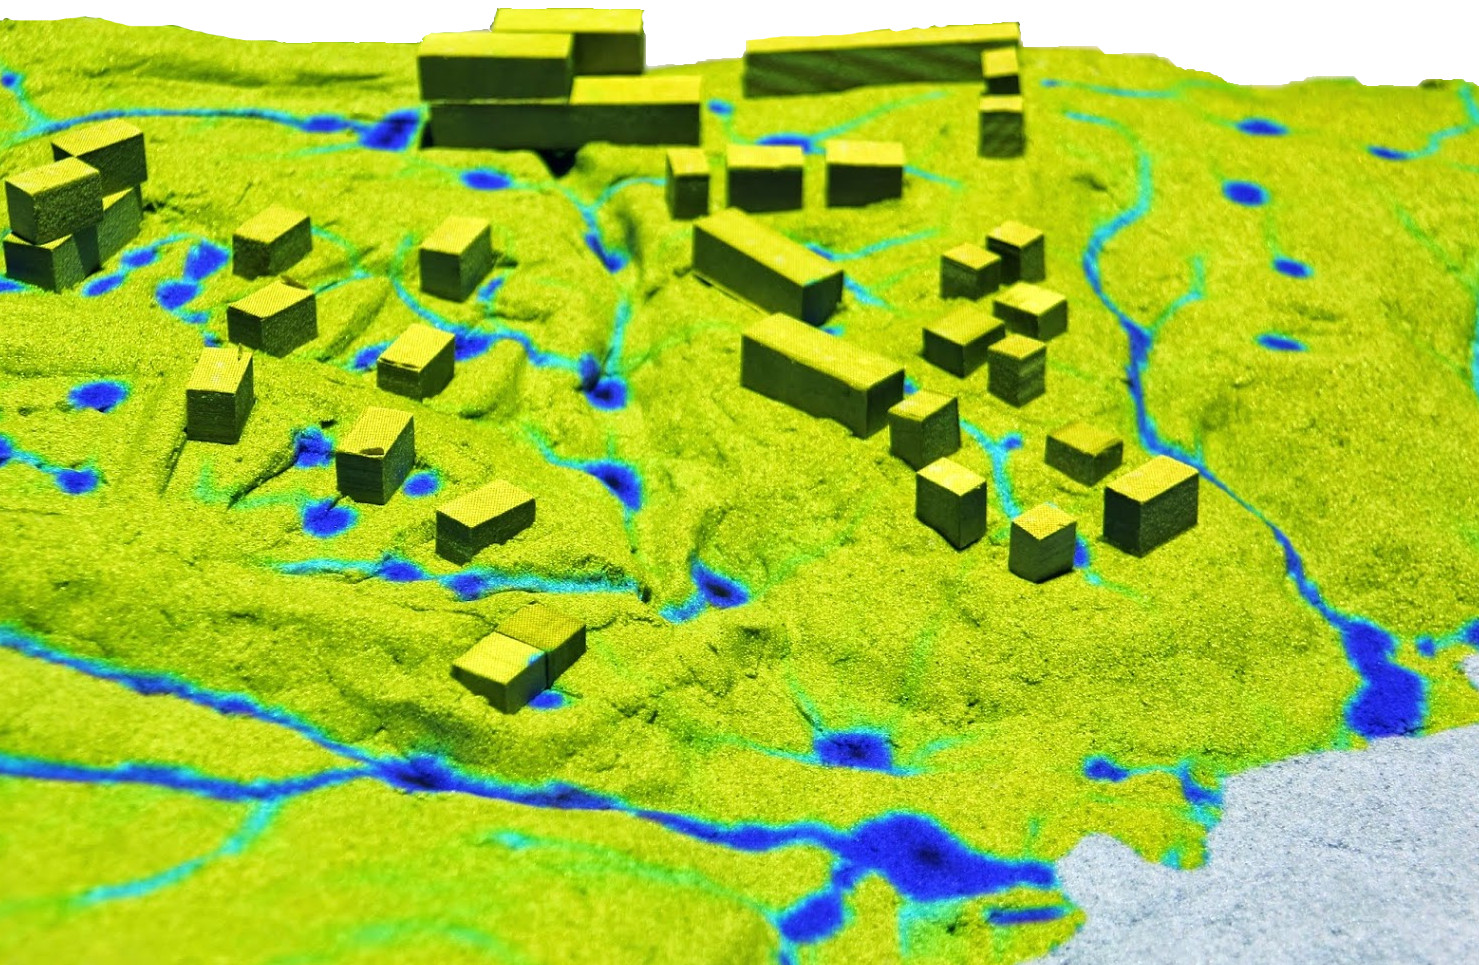
\includegraphics[width=\textwidth]{rsimwater_architects}

\textcolor{gray}{
\footnotesize
Overland water flow simulated by \gmodule{r.sim.water}
\\
in \emph{Tangible Landscape} environment
}

\end{column}
\end{columns}

\end{frame}


%%%%%%%%%%%%%%%%%%%%%%%%%%%%%%%%%%%%%%%%%%%%%%%%%%%%%%%%%%%%%%%%%%%%%
\begin{frame}{Code is further developed by other contributors}

\begin{columns}
\begin{column}{0.5\textwidth}

\begin{itemize}
  \item least cost path flow tracing (Ehlschlaeger 1989) extended by Markus Metz
  \item interpolation using splines (Mitasova \& Mitas 1993) was parallelized (Hofierka et al. 2017)
\end{itemize}


\bigskip
\footnoterule
\tiny

Ehlschlaeger C. (1989). Using the $A^T$ Search Algorithm to Develop Hydrologic Models from Digital Elevation Data, Proceedings of International Geographic Information Systems (IGIS) Symposium '89, pp 275-281 (Baltimore, MD, 18-19 March 1989).

Mitasova, H. and Mitas, L. (1993) Interpolation by Regularized Spline with Tension: I. Theory and Implementation, Mathematical Geology, 25, 641-655.

Hofierka, J., Lacko, M., and Zubal, S. (2017). Parallelization of interpolation, solar radiation and water flow simulation modules in GRASS GIS using OpenMP. Computers \& Geosciences, 107, 20-27.

\end{column}
\begin{column}{0.5\textwidth}
\centering
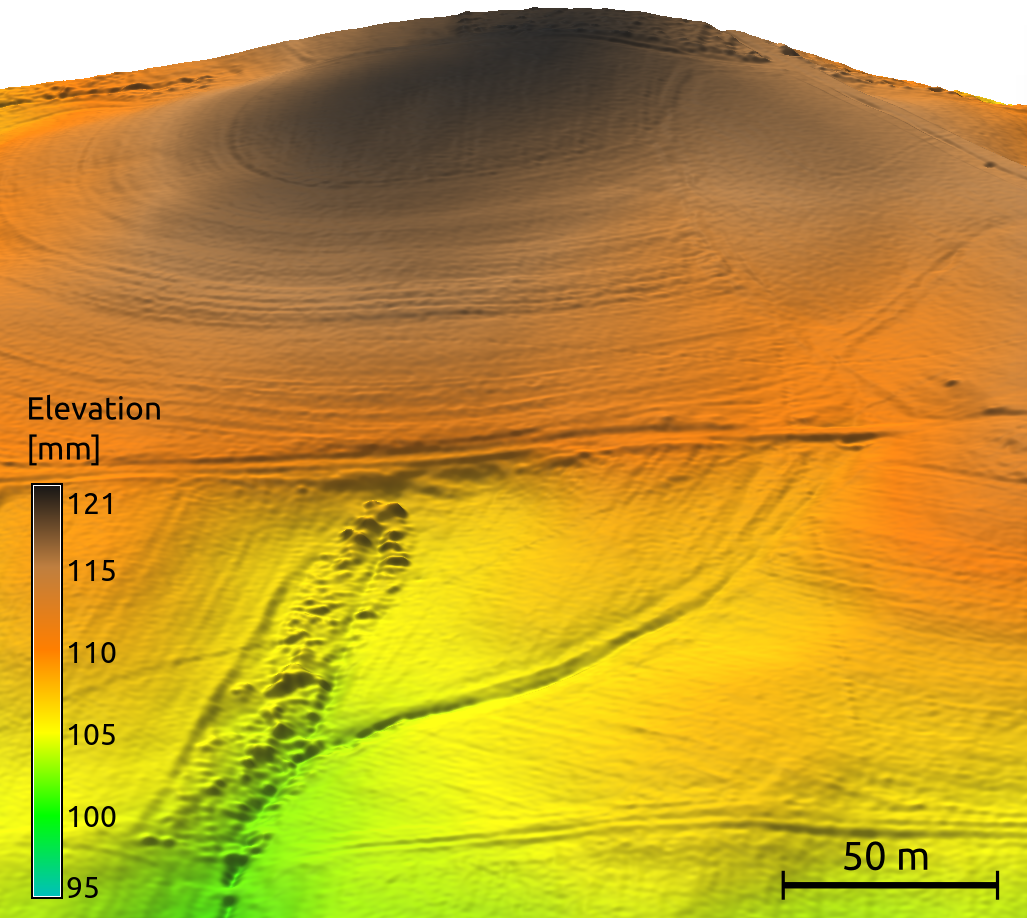
\includegraphics[width=\textwidth]{elevation_lidar}

\textcolor{gray}{
\footnotesize
Digital elevation model interpolated by \gmodule{v.surf.rst}
}

\end{column}
\end{columns}

\end{frame}


%%%%%%%%%%%%%%%%%%%%%%%%%%%%%%%%%%%%%%%%%%%%%%%%%%%%%%%%%%%%%%%%%%%%%
\begin{frame}{Algorithms published elsewhere are available}

\begin{columns}
\begin{column}{0.5\textwidth}

\begin{itemize}
  \item Multiscale Curvature Classification (Evans \& Hudak 2007) implemented by Stefan Blumentrath
  % this is also an example of reuse of code inside GRASS
  \item SLIC Superpixels segmentation (Achanta et al. 2012) implemented by Rashad Kanavath and Markus Metz
\end{itemize}

\bigskip
\footnoterule
\tiny

Evans, J. S. and Hudak, A. T. (2007) A Multiscale Curvature Algorithm for Classifying Discrete Return LiDAR in Forested Environments. IEEE Transactions on Geoscience and Remote Sensing 45(4): 1029 - 1038

Achanta, R., Shaji, A., Smith, K., Lucchi, A., Fua, P., and Süsstrunk, S. (2012). SLIC superpixels compared to state-of-the-art superpixel methods. IEEE transactions on pattern analysis and machine intelligence, 34(11):2274–2282.

\end{column}

\begin{column}{0.5\textwidth}
\centering
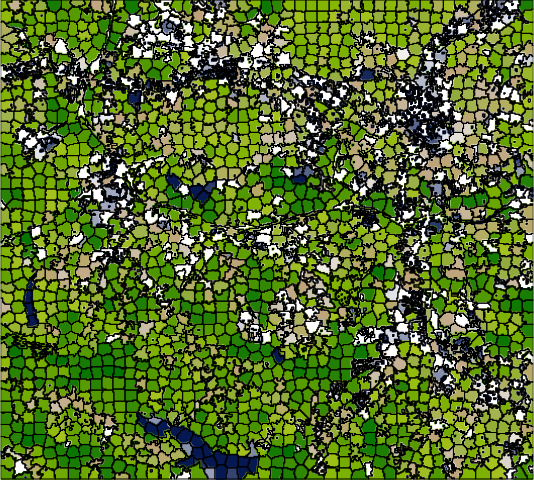
\includegraphics[width=\textwidth]{i_superpixels_slic_ndvi}

\textcolor{gray}{
\footnotesize
Superpixels by \gmodule{i.superpixels.slic} and NDVI by \gmodule{i.vi}
}

\end{column}
\end{columns}

\end{frame}


%%%%%%%%%%%%%%%%%%%%%%%%%%%%%%%%%%%%%%%%%%%%%%%%%%%%%%%%%%%%%%%%%%%%%
\begin{frame}{Publishing code through GRASS GIS}

\begin{block}{}
 \begin{itemize}
  \item Ask for access to GRASS GIS Addons at
        \\
        \href{https://grass.osgeo.org/development/code-submission/}{\texttt{grass.osgeo.org/development/code-submission}}
  \item Example GRASS GIS module
        \\
        \href{https://gitlab.com/vpetras/r.example.plus/}{\texttt{gitlab.com/vpetras/r.example.plus}}
 \end{itemize}
\end{block}

\bigskip
\centering

\begin{tabular}{clc}
\begin{minipage}{0.16\textwidth}

\includegraphics[width=\textwidth]{grass_gis}
\end{minipage}
&
\begin{minipage}{0.5\textwidth}
\footnotesize
\href{https://grass.osgeo.org}{%
Get GRASS GIS at\\
\texttt{grass.osgeo.org}%
}

\bigskip

{
\footnotesize
\href{https://lists.osgeo.org/listinfo/grass-user}{GRASS user mailing list}\\
\href{https://lists.osgeo.org/listinfo/grass-user}{\texttt{lists.osgeo.org/listinfo/grass-user}}
}

\bigskip

{
\footnotesize
Source files for posters and slides available at\\
\href{https://trac.osgeo.org/grass/browser/grass-promo/}%
  {\texttt{trac.osgeo.org/grass/browser/grass-promo}}
}
\end{minipage}
&
\begin{minipage}{0.2\textwidth}
% \includegraphics[width=\textwidth]{talks_qr}
\end{minipage}
\end{tabular}

\end{frame}

% don't count the backup and ack slides
\backupbegin

%%%%%%%%%%%%%%%%%%%%%%%%%%%%%%%%%%%%%%%%%%%%%%%%%%%%%%%%%%%%%%%%%%%%%
\begin{frame}{Acknowledgements}

\footnotesize

\begin{columns}
\begin{column}{0.6\textwidth}

\begin{block}{Software \& community}
The GRASS GIS Development Team, contributors, users, ...
\end{block}

\begin{block}{Datasets}

% \smallskip

Nantahala NF, NC: Forest Leaf Structure, Terrain and Hydrophysiology.
% Lidar data acquisition and processing completed
% by the National Center for Airborne Laser Mapping (\href{http://www.ncalm.org}{NCALM}).
% NCALM funding provided by NSF's Division of Earth Sciences, Instrumentation and Facilities Program.
% EAR-1043051.
Obtained from \href{http://www.opentopography.org/}{OpenTopography}.
\url{https://doi.org/10.5069/G9HT2M76}

Dataset for North Carolina State University GIS595-005/603; MEA592-004/601: UAS Mapping for 3D Modeling

North Carolina Sample Dataset for GRASS GIS
\end{block}

\begin{block}{Presentation software}
Slides were created in \textrm{\LaTeX{}} using the~\textrm{\textsc{beamer} \textit{class}}.
% all lowercase, sc and it taken from the beamer user guide
\end{block}


\end{column}
\begin{column}{0.3\textwidth}

\begin{center}
  
\includegraphics[width=\textwidth]{logos/grass_gis}
\end{center}

\end{column}
\end{columns}

\end{frame}

\backupend

\end{document}
